\upaper{35}{The Local Universe Sons of God}
\uminitoc{The Father Melchizedek}
\uminitoc{The Melchizedek Sons}
\uminitoc{The Melchizedek Worlds}
\uminitoc{Special Work of the Melchizedeks}
\uminitoc{The Vorondadek Sons}
\uminitoc{The Constellation Fathers}
\uminitoc{The Vorondadek Worlds}
\uminitoc{The Lanonandek Sons}
\uminitoc{The Lanonandek Rulers}
\uminitoc{The Lanonandek Worlds}
\author{Chief of Archangels}
\vs p035 0:1 The Sons of God previously introduced have had a Paradise origin. They are the offspring of the divine Rulers of the universal domains. Of the first Paradise order of sonship, the Creator Sons, there is in Nebadon only one, Michael, the universe father and sovereign. Of the second order of Paradise sonship, the Avonal or Magisterial Sons, Nebadon has its full quota --- 1,062. And these “lesser Christs” are just as effective and all\hyp{}powerful in their planetary bestowals as was the Creator and Master Son on Urantia. The third order, being of Trinity origin, do not register in a local universe, but I estimate there are in Nebadon between 15,000 and 20,000 Trinity Teacher Sons exclusive of 9,642 creature\hyp{}trinitized assistants of record. These Paradise Daynals are neither magistrates nor administrators; they are superteachers.
\vs p035 0:2 The types of Sons about to be considered are of local universe origin; they are the offspring of a Paradise Creator Son in varied association with the complemental Universe Mother Spirit. The following orders of local universe sonship find mention in these narratives:
\vs p035 0:3 \ublistelem{1.}\bibnobreakspace Melchizedek Sons.
\vs p035 0:4 \ublistelem{2.}\bibnobreakspace Vorondadek Sons.
\vs p035 0:5 \ublistelem{3.}\bibnobreakspace Lanonandek Sons.
\vs p035 0:6 \ublistelem{4.}\bibnobreakspace Life Carrier Sons.
\vs p035 0:7 \pc Triune Paradise Deity functions for the creation of three orders of sonship: the Michaels, the Avonals, and the Daynals. Dual Deity in the local universe, the Son and the Spirit, also functions in the creation of three high orders of Sons: the Melchizedeks, the Vorondadeks, and the Lanonandeks; and having achieved this threefold expression, they collaborate with the next level of God the Sevenfold in the production of the versatile order of Life Carriers. These beings are classified with the descending Sons of God, but they are a unique and original form of universe life. Their consideration will occupy the whole of the next paper.
\usection{The Father Melchizedek}
\vs p035 1:1 After bringing into existence the beings of personal aid, such as the Bright and Morning Star and other administrative personalities, in accordance with the divine purpose and creative plans of a given universe, there occurs a new form of creative union between the Creator Son and the Creative Spirit, the local universe Daughter of the Infinite Spirit. The personality offspring resulting from this creative partnership is the original Melchizedek --- the Father Melchizedek --- that unique being who subsequently collaborates with the Creator Son and the Creative Spirit to bring into existence the entire group of that name.
\vs p035 1:2 In the universe of Nebadon the Father Melchizedek acts as the first executive associate of the Bright and Morning Star. Gabriel is occupied more with universe policies, Melchizedek with practical procedures. Gabriel presides over the regularly constituted tribunals and councils of Nebadon, Melchizedek over the special, extraordinary, and emergency commissions and advisory bodies. Gabriel and the Father Melchizedek are never away from Salvington at the same time\fnst{They were \bibemph{apparently} away at the same time on the Mount of Transfiguration, cf. \bibref[158:1.6,7]{p158 1:6}.}, for in Gabriel’s absence the Father Melchizedek functions as the chief executive of Nebadon.
\vs p035 1:3 The Melchizedeks of our universe were all created within one millennial period of standard time by the Creator Son and the Creative Spirit in liaison with the Father Melchizedek. Being an order of sonship wherein one of their own number functioned as co\hyp{}ordinate creator, Melchizedeks are in constitution partly of self\hyp{}origin and therefore candidates for the realization of a supernal type of self\hyp{}government. They periodically elect their own administrative chief for a term of 7 years of standard time and otherwise function as a self\hyp{}regulating order, though the original Melchizedek does exercise certain inherent coparental prerogatives. From time to time this Father Melchizedek designates certain individuals of his order to function as special Life Carriers to the midsonite worlds, a type of inhabited planet not heretofore revealed on Urantia.
\vs p035 1:4 The Melchizedeks do not function extensively outside the local universe except when they are called as witnesses in matters pending before the tribunals of the superuniverse, and when designated special ambassadors, as they sometimes are, representing one universe to another in the same superuniverse. The original or first\hyp{}born Melchizedek of each universe is always at liberty to journey to the neighbouring universes or to Paradise on missions having to do with the interests and duties of his order.
\usection{The Melchizedek Sons}
\vs p035 2:1 The Melchizedeks are the first order of divine Sons to approach sufficiently near the lower creature life to be able to function directly in the ministry of mortal uplift, to serve the evolutionary races without the necessity of incarnation. These Sons are naturally at the mid\hyp{}point of the great personality descent, by origin being just about midway between the highest Divinity and the lowest creature life of will endowment. They thus become the natural intermediaries between the higher and divine levels of living existence and the lower, even the material, forms of life on the evolutionary worlds. The seraphic orders, the angels, delight to work with the Melchizedeks; in fact, all forms of intelligent life find in these Sons understanding friends, sympathetic teachers, and wise counsellors.
\vs p035 2:2 The Melchizedeks are a self\hyp{}governing order. With this unique group we encounter the first attempt at self\hyp{}determination on the part of local universe beings and observe the highest type of true self\hyp{}government. These Sons organize their own machinery for their group and home\hyp{}planet administration, as well as that for the 6 associated spheres and their tributary worlds. And it should be recorded that they have never abused their prerogatives; not once throughout all the superuniverse of Orvonton have these Melchizedek Sons ever betrayed their trust. They are the hope of every universe group which aspires to self\hyp{}government; they are the pattern and the teachers of self\hyp{}government to all the spheres of Nebadon. All orders of intelligent beings, superiors from above and subordinates from below, are wholehearted in their praise of the government of the Melchizedeks.
\vs p035 2:3 \pc The Melchizedek order of sonship occupies the position, and assumes the responsibility, of the eldest son in a large family. Most of their work is regular and somewhat routine, but much of it is voluntary and altogether self\hyp{}imposed. A majority of the special assemblies which, from time to time, convene on Salvington are called on motion of the Melchizedeks. On their own initiative these Sons patrol their native universe. They maintain an autonomous organization devoted to universe intelligence, making periodical reports to the Creator Son independent of all information coming up to universe headquarters through the regular agencies concerned with the routine administration of the realm. They are by nature unprejudiced observers; they have the full confidence of all classes of intelligent beings.
\vs p035 2:4 The Melchizedeks function as mobile and advisory review courts of the realms; these universe Sons go in small groups to the worlds to serve as advisory commissions, to take depositions, to receive suggestions, and to act as counsellors, thus helping to compose the major difficulties and settle the serious differences which arise from time to time in the affairs of the evolutionary domains.
\vs p035 2:5 These eldest Sons of a universe are the chief aids of the Bright and Morning Star in carrying out the mandates of the Creator Son. When a Melchizedek goes to a remote world in the name of Gabriel, he may, for the purposes of that particular mission, be deputized in the name of the sender and in that event will appear on the planet of assignment with the full authority of the Bright and Morning Star. Especially is this true on those spheres where a higher Son has not yet appeared in the likeness of the creatures of the realm.
\vs p035 2:6 When a Creator Son enters upon the bestowal career on an evolutionary world, he goes alone; but when one of his Paradise brothers, an Avonal Son, enters upon a bestowal, he is accompanied by the Melchizedek supporters, 12 in number, who so efficiently contribute to the success of the bestowal mission. They also support the Paradise Avonals on magisterial missions to the inhabited worlds, and in these assignments the Melchizedeks are visible to mortal eyes if the Avonal Son is also thus manifest.
\vs p035 2:7 There is no phase of planetary spiritual need to which they do not minister. They are the teachers who so often win whole worlds of advanced life to the final and full recognition of the Creator Son and his Paradise Father.
\vs p035 2:8 \pc The Melchizedeks are well\hyp{}nigh perfect in wisdom, but they are not infallible in judgment. When detached and alone on planetary missions, they have sometimes erred in minor matters, that is, they have elected to do certain things which their supervisors did not subsequently approve. Such an error of judgment temporarily disqualifies a Melchizedek until he goes to Salvington and, in audience with the Creator Son, receives that instruction which effectually purges him of the disharmony which caused disagreement with his fellows; and then, following the correctional rest, reinstatement to service ensues on the third day. But these minor misadaptations in Melchizedek function have rarely occurred in Nebadon.
\vs p035 2:9 These Sons are not an increasing order; their number is stationary, although varying in each local universe. The number of Melchizedeks of record on their headquarters planet in Nebadon is upward of 10,000,000.
\usection{The Melchizedek Worlds}
\vs p035 3:1 The Melchizedeks occupy a world of their own near Salvington, the universe headquarters. This sphere, by name Melchizedek, is the pilot world of the Salvington circuit of 70 primary spheres, each of which is encircled by 6 tributary spheres devoted to specialized activities. These marvellous spheres --- 70 primaries and 420 tributaries --- are often spoken of as the Melchizedek University. Ascending mortals from all the constellations of Nebadon pass through training on all 490 worlds in the acquirement of residential status on Salvington. But the education of ascenders is only one phase of the manifold activities taking place on the Salvington cluster of architectural spheres.
\vs p035 3:2 The 490 spheres of the Salvington circuit are divided into 10 groups, each containing 7 primary and 42 tributary spheres. Each of these groups is under the general supervision of some one of the major orders of universe life. The first group, embracing the pilot world and the next 6 primary spheres in the encircling planetary procession, is under the supervision of the Melchizedeks. These Melchizedek worlds are:\tunemarkup{pictures}{\begin{figure}[H]\centering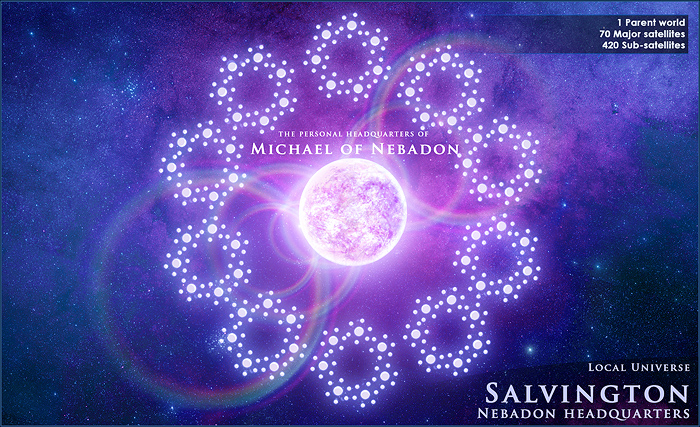
\includegraphics[angle=90,width=\tunemarkup{pgkoboaurahd}{0.7}\tunemarkup{pgnexus10}{0.9}\columnwidth]{images/SALVINGTON-700.jpg}\caption{Salvington by Gary Tonge}\end{figure}}
\vs p035 3:3 \ublistelem{1.}\bibnobreakspace The pilot world --- the home world of the Melchizedek Sons.
\vs p035 3:4 \ublistelem{2.}\bibnobreakspace The world of the physical\hyp{}life schools and the laboratories of living energies.
\vs p035 3:5 \ublistelem{3.}\bibnobreakspace The world of morontia life.
\vs p035 3:6 \ublistelem{4.}\bibnobreakspace The sphere of initial spirit life.
\vs p035 3:7 \ublistelem{5.}\bibnobreakspace The world of mid\hyp{}spirit life.
\vs p035 3:8 \ublistelem{6.}\bibnobreakspace The sphere of advancing spirit life.
\vs p035 3:9 \ublistelem{7.}\bibnobreakspace The domain of co\hyp{}ordinate and supreme self\hyp{}realization.
\vs p035 3:10 \pc The 6 tributary worlds of each of these Melchizedek spheres are devoted to activities germane to the work of the associated primary sphere.
\vs p035 3:11 \pc The pilot world, the sphere \bibemph{Melchizedek,} is the common meeting ground for all beings who are engaged in educating and spiritualizing the ascending mortals of time and space. To an ascender this world is probably the most interesting place in all Nebadon. All evolutionary mortals who graduate from their constellation training are destined to land on Melchizedek, where they are initiated into the regime of the disciplines and spirit progression of the Salvington educational system. And never will you forget your reactions to the first day of life on this unique world, not even after you have reached your Paradise destination.
\vs p035 3:12 Ascending mortals maintain residence on the Melchizedek world while pursuing their training on the 6 encircling planets of specialized education. And this same method is adhered to throughout their sojourn on the 70 cultural worlds, the primary spheres of the Salvington circuit.
\vs p035 3:13 \pc Many diverse activities occupy the time of the numerous beings who reside on the 6 tributary worlds of the Melchizedek sphere, but as concerns the ascending mortals, these satellites are devoted to the following special phases of study:
\vs p035 3:14 \ublistelem{1.}\bibnobreakspace Sphere number one is occupied with the review of the initial planetary life of the ascending mortals. This work is carried on in classes composed of those who hail from a given world of mortal origin. Those from Urantia pursue such an experiential review together.
\vs p035 3:15 \ublistelem{2.}\bibnobreakspace The special work of sphere number two consists in a similar review of the experiences passed through on the mansion worlds encircling the premier satellite of the local system headquarters.
\vs p035 3:16 \ublistelem{3.}\bibnobreakspace The reviews of this sphere pertain to the sojourn on the capital of the local system and embrace the activities of the remainder of the architectural worlds of the system headquarters cluster.
\vs p035 3:17 \ublistelem{4.}\bibnobreakspace The fourth sphere is occupied with a review of the experiences of the 70 tributary worlds of the constellation and of their associated spheres.
\vs p035 3:18 \ublistelem{5.}\bibnobreakspace On the fifth sphere there is conducted the review of the ascendant sojourn on the constellation headquarters world.
\vs p035 3:19 \ublistelem{6.}\bibnobreakspace The time on sphere number six is devoted to an attempt to correlate these five epochs and thus achieve co\hyp{}ordination of experience preparatory to entering the Melchizedek primary schools of universe training.
\vs p035 3:20 \pc The schools of universe administration and spiritual wisdom are located on the Melchizedek home world, where also are to be found those schools devoted to a single line of research, such as energy, matter, organization, communication, records, ethics, and comparative creature existence.
\vs p035 3:21 In the Melchizedek College of Spiritual Endowment all orders --- even the Paradise orders --- of the Sons of God co\hyp{}operate with the Melchizedek and the seraphic teachers in training the hosts who go forth as evangels of destiny, proclaiming spiritual liberty and divine sonship even to the remote worlds of the universe. This particular school of the Melchizedek University is an exclusive universe institution; student visitors are not received from other realms.
\vs p035 3:22 The highest course of training in universe administration is given by the Melchizedeks on their home world. This College of High Ethics is presided over by the original Father Melchizedek. It is to these schools that the various universes send exchange students. While the young universe of Nebadon stands low in the scale of universes as regards spiritual achievement and high ethical development, nevertheless, our administrative troubles have so turned the whole universe into a vast clinic for other near\hyp{}by creations that the Melchizedek colleges are thronged with student visitors and observers from other realms. Besides the immense group of local registrants there are always upward of 100,000 foreign students in attendance upon the Melchizedek schools, for the order of Melchizedeks in Nebadon is renowned throughout all Splandon.
\usection{Special Work of the Melchizedeks}
\vs p035 4:1 A highly specialized branch of Melchizedek activities has to do with the supervision of the progressive morontia career of the ascending mortals. Much of this training is conducted by the patient and wise seraphic ministers, assisted by mortals who have ascended to relatively higher levels of universe attainment, but all of this educational work is under the general supervision of the Melchizedeks in association with the Trinity Teacher Sons.
\vs p035 4:2 \pc While the Melchizedek orders are chiefly devoted to the vast educational system and experiential training regime of the local universe, they also function in unique assignments and in unusual circumstances. In an evolving universe eventually embracing approximately 10,000,000 inhabited worlds, many things out of the ordinary are destined to happen, and it is in such emergencies that the Melchizedeks act. On Edentia, your constellation headquarters, they are known as emergency Sons. They are always ready to serve in all exigencies --- physical, intellectual, or spiritual --- whether on a planet, in a system, in a constellation, or in the universe. Whenever and wherever special help is needed, there you will find one or more of the Melchizedek Sons.
\vs p035 4:3 When failure of some feature of the Creator Son’s plan is threatened, forthwith will go a Melchizedek to render assistance. But not often are they summoned to function in the presence of sinful rebellion, such as occurred in Satania.
\vs p035 4:4 The Melchizedeks are the first to act in all emergencies of whatever nature on all worlds where will creatures dwell. They sometimes act as temporary custodians on wayward planets, serving as receivers of a defaulting planetary government. In a planetary crisis these Melchizedek Sons serve in many unique capacities. It is easily possible for such a Son to make himself visible to mortal beings, and sometimes one of this order has even incarnated in the likeness of mortal flesh. Seven times in Nebadon has a Melchizedek served on an evolutionary world in the similitude of mortal flesh, and on numerous occasions these Sons have appeared in the likeness of other orders of universe creatures. They are indeed the versatile and volunteer emergency ministers to all orders of universe intelligences and to all the worlds and systems of worlds.
\vs p035 4:5 \pc The Melchizedek who lived on Urantia during the time of Abraham was locally known as Prince of Salem because he presided over a small colony of truth seekers residing at a place called Salem. He volunteered to incarnate in the likeness of mortal flesh and did so with the approval of the Melchizedek receivers of the planet, who feared that the light of life would become extinguished during that period of increasing spiritual darkness. And he did foster the truth of his day and safely pass it on to Abraham and his associates.
\usection{The Vorondadek Sons}
\vs p035 5:1 After the creation of the personal aids and the first group of the versatile Melchizedeks, the Creator Son and the local universe Creative Spirit planned for, and brought into existence, the second great and diverse order of universe sonship, the Vorondadeks. They are more generally known as Constellation Fathers because a Son of this order is uniformly found at the head of each constellation government in every local universe.
\vs p035 5:2 \pc The number of Vorondadeks varies in each local universe, just 1,000,000 being the recorded number in Nebadon. These Sons, like their co\hyp{}ordinates, the Melchizedeks, possess no power of reproduction. There exists no known method whereby they can increase their numbers.
\vs p035 5:3 \pc In many respects these Sons are a self\hyp{}governing body; as individuals and as groups, even as a whole, they are largely self\hyp{}determinative, much as are the Melchizedeks, but Vorondadeks do not function through such a wide range of activities. They do not equal their Melchizedek brethren in brilliant versatility, but they are even more reliable and efficient as rulers and farseeing administrators. Neither are they quite the administrative peers of their subordinates, the Lanonandek System Sovereigns, but they excel all orders of universe sonship in stability of purpose and in divinity of judgment.
\vs p035 5:4 Although the decisions and rulings of this order of Sons are always in accordance with the spirit of divine sonship and in harmony with the policies of the Creator Son, they have been cited for error to the Creator Son, and in details of technique their decisions have sometimes been reversed on appeal to the superior tribunals of the universe. But these Sons rarely fall into error, and they have never gone into rebellion; never in all the history of Nebadon has a Vorondadek been found in contempt of the universe government.
\vs p035 5:5 The service of the Vorondadeks in the local universes is extensive and varied. They serve as ambassadors to other universes and as consuls representing constellations within their native universe. Of all orders of local universe sonship they are the most often entrusted with the full delegation of sovereign powers to be exercised in critical universe situations.
\vs p035 5:6 On those worlds segregated in spiritual darkness, those spheres which have, through rebellion and default, suffered planetary isolation, an observer Vorondadek is usually present pending the restoration of normal status. In certain emergencies this Most High observer could exercise absolute and arbitrary authority over every celestial being assigned to that planet. It is of record on Salvington that the Vorondadeks have sometimes exercised such authority as Most High regents of such planets. And this has also been true even of inhabited worlds that were untouched by rebellion.
\vs p035 5:7 Often a corps of 12 or more Vorondadek Sons sits en banc\fnst{As a group, particularly with respect to a legal decision rendered by all of the judges sitting on a court, rather than by a smaller panel of judges from that court.} as a high court of review and appeal concerning special cases involving the status of a planet or a system. But their work more largely pertains to the legislative functions indigenous to the constellation governments. As a result of all these services, the Vorondadek Sons have become the historians of the local universes; they are personally familiar with all the political struggles and the social upheavals of the inhabited worlds.
\usection{The Constellation Fathers}
\vs p035 6:1 At least three Vorondadeks are assigned to the rulership of each of the 100 constellations of a local universe. These Sons are selected by the Creator Son and are commissioned by Gabriel as the \bibemph{Most Highs} of the constellations for service during one dekamillennium --- 10,000 standard years, about 50,000 years of Urantia time. The reigning Most High, the Constellation Father, has two associates, a senior and a junior. At each change of administration the senior associate becomes the head of the government, the junior assumes the duties of the senior, while the unassigned Vorondadeks resident on the Salvington worlds nominate one of their number as candidate for selection to assume the responsibilities of junior associate. Thus each of the Most High rulers, in accordance with present policy, has a period of service on the headquarters of a constellation of three dekamillenniums, about 150,000 Urantia years.
\vs p035 6:2 The 100 Constellation Fathers, the actual presiding heads of the constellation governments, constitute the supreme advisory cabinet of the Creator Son. This council is in frequent session at universe headquarters and is unlimited in the scope and range of its deliberations but is chiefly concerned with the welfare of the constellations and with the unification of the administration of the entire local universe.
\vs p035 6:3 When a Constellation Father is in attendance upon duties at the universe headquarters, as he frequently is, the senior associate becomes acting director of constellation affairs. The normal function of the senior associate is the oversight of spiritual affairs, while the junior associate is personally occupied with the physical welfare of the constellation. No major policy, however, is ever carried out in a constellation unless all three of the Most Highs are agreed upon all the details of its execution.
\vs p035 6:4 The entire mechanism of spirit intelligence and communication channels is at the disposal of the constellation Most Highs. They are in perfect touch with their superiors on Salvington and with their direct subordinates, the sovereigns of the local systems. They frequently convene in council with these System Sovereigns to deliberate upon the state of the constellation.
\vs p035 6:5 The Most Highs surround themselves with a corps of counsellors, which varies in number and personnel from time to time in accordance with the presence of the various groups at constellation headquarters and also as the local requirements vary. During times of stress they may ask for, and will quickly receive, additional Sons of the Vorondadek order to assist with the administrative work. Norlatiadek, your own constellation, is at present administered by 12 Vorondadek Sons.
\usection{The Vorondadek Worlds}
\vs p035 7:1 The second group of 7 worlds in the circuit of 70 primary spheres surrounding Salvington comprise the Vorondadek planets. Each of these spheres, with its 6 encircling satellites, is devoted to a special phase of Vorondadek activities. On these 49 realms the ascending mortals secure the acme of their education respecting universe legislation.
\vs p035 7:2 The ascending mortals have observed the legislative assemblies as they functioned on the headquarters worlds of the constellations, but here on these Vorondadek worlds they participate in the enactment of the actual general legislation of the local universe under the tutelage of the senior Vorondadeks. Such enactments are designed to co\hyp{}ordinate the varied pronouncements of the autonomous legislative assemblies of the 100 constellations. The instruction to be had in the Vorondadek schools is unexcelled even on Uversa. This training is progressive, extending from the first sphere, with supplemental work on its 6 satellites, on up through the remaining 6 primary spheres and their associated satellite groups.
\vs p035 7:3 The ascending pilgrims will be introduced to numerous new activities on these worlds of study and practical work. We are not forbidden to undertake the revelation of these new and undreamed\hyp{}of pursuits, but we despair of being able to portray these undertakings to the material mind of mortal beings. We are without words to convey the meanings of these supernal activities, and there are no analogous human engagements which might be utilized as illustrations of these new occupations of the ascending mortals as they pursue their studies on these 49 worlds. And many other activities, not a part of the ascendant regime, are centred on these Vorondadek worlds of the Salvington circuit.
\usection{The Lanonandek Sons}
\vs p035 8:1 After the creation of the Vorondadeks, the Creator Son and the Universe Mother Spirit unite for the purpose of bringing into existence the third order of universe sonship, the Lanonandeks. Although occupied with varied tasks connected with the system administrations, they are best known as System Sovereigns, the rulers of the local systems, and as Planetary Princes, the administrative heads of the inhabited worlds.
\vs p035 8:2 Being a later and lower --- as concerns divinity levels --- order of sonship creation, these beings were required to pass through certain courses of training on the Melchizedek worlds in preparation for subsequent service. They were the first students in the Melchizedek University and were classified and certified by their Melchizedek teachers and examiners according to ability, personality, and attainment.
\vs p035 8:3 The universe of Nebadon began its existence with exactly 12,000,000 Lanonandeks, and when they had passed through the Melchizedek sphere, they were divided in the final tests into three classes:
\vs p035 8:4 \ublistelem{1.}\bibnobreakspace \bibemph{Primary Lanonandeks.} Of the highest rank there were 709,841. These are the Sons designated as System Sovereigns and assistants to the supreme councils of the constellations and as counsellors in the higher administrative work of the universe.
\vs p035 8:5 \ublistelem{2.}\bibnobreakspace \bibemph{Secondary Lanonandeks.} Of this order emerging from Melchizedek there were 10,234,601. They are assigned as Planetary Princes and to the reserves of that order.
\vs p035 8:6 \ublistelem{3.}\bibnobreakspace \bibemph{Tertiary Lanonandeks.} This group contained 1,055,558. These Sons function as subordinate assistants, messengers, custodians, commissioners, observers, and prosecute the miscellaneous duties of a system and its component worlds.
\vs p035 8:7 \pc It is not possible, as it is with evolutionary beings, for these Sons to progress from one group to another. When subjected to the Melchizedek training, when once tested and classified, they serve continuously in the rank assigned. Neither do these Sons engage in reproduction; their number in the universe is stationary.
\vs p035 8:8 In round numbers the Lanonandek order of Sons is classified on Salvington as follows:
\vs p035 8:9 \pc Universe Co\hyp{}ordinators and Constellation\tunemarkup{pgauraone}{\linebreak} Counsellors\bibdf100,000
\vs p035 8:10 System Sovereigns and Assistants\bibdf600,000
\vs p035 8:11 Planetary Princes and Reserves\bibdf10,000,000
\vs p035 8:12 Messenger Corps\bibdf400,000
\vs p035 8:13 Custodians and Recorders\bibdf100,000
\vs p035 8:14 Reserve Corps\bibdf800,000
\vs p035 8:15 \pc Since Lanonandeks are a somewhat lower order of sonship than the Melchizedeks and the Vorondadeks, they are of even greater service in the subordinate units of the universe, for they are capable of drawing nearer the lower creatures of the intelligent races. They also stand in greater danger of going astray, of departing from the acceptable technique of universe government. But these Lanonandeks, especially the primary order, are the most able and versatile of all local universe administrators. In executive ability they are excelled only by Gabriel and his unrevealed associates.
\usection{The Lanonandek Rulers}
\vs p035 9:1 The Lanonandeks are the continuous rulers of the planets and the rotating sovereigns of the systems. Such a Son now rules on Jerusem, the headquarters of your local system of inhabited worlds.
\vs p035 9:2 The System Sovereigns rule in commissions of two or three on the headquarters of each system of inhabited worlds. The Constellation Father names one of these Lanonandeks as chief every dekamillennium. Sometimes no change in the head of the trio is made, the matter being entirely optional with the constellation rulers. System governments do not suddenly change in personnel unless a tragedy of some sort occurs.
\vs p035 9:3 When System Sovereigns or assistants are recalled, their places are filled by selections made by the supreme council located on the constellation headquarters from the reserves of that order, a group which is larger on Edentia than the average indicated.
\vs p035 9:4 The supreme Lanonandek councils are stationed on the various constellation headquarters. Such a body is presided over by the senior Most High associate of the Constellation Father, while the junior associate supervises the reserves of the secondary order.
\vs p035 9:5 \pc The System Sovereigns are true to their names; they are well\hyp{}nigh sovereign in the local affairs of the inhabited worlds. They are almost paternal in their direction of the Planetary Princes, the Material Sons, and the ministering spirits. The personal grasp of the sovereign is all but complete. These rulers are not supervised by Trinity observers from the central universe. They are the executive division of the local universe, and as custodians of the enforcement of legislative mandates and as executives for the application of judicial verdicts, they present the one place in all universe administration where personal disloyalty to the will of the Michael Son could most easily and readily entrench itself and seek to assert itself.
\vs p035 9:6 Our local universe has been unfortunate in that over 700 Sons of the Lanonandek order have rebelled against the universe government, thus precipitating confusion in several systems and on numerous planets. Of this entire number of failures only three were System Sovereigns; practically all of these Sons belonged to the second and third orders, Planetary Princes and tertiary Lanonandeks.
\vs p035 9:7 The large number of these Sons who have lapsed from integrity does not indicate any fault in creatorship. They could have been made divinely perfect, but they were so created that they might better understand, and draw near to, the evolutionary creatures dwelling on the worlds of time and space.
\vs p035 9:8 Of all the local universes in Orvonton, our universe has, with the exception of Henselon, lost the largest number of this order of Sons. On Uversa it is the consensus that we have had so much administrative trouble in Nebadon because our Sons of the Lanonandek order have been created with such a large degree of personal liberty in choosing and planning. I do not make this observation by way of criticism. The Creator of our universe has full authority and power to do this. It is the contention of our high rulers that, while such free\hyp{}choosing Sons make excessive trouble in the earlier ages of the universe, when things are fully sifted and finally settled, the gains of higher loyalty and fuller volitional service on the part of these thoroughly tested Sons will far more than compensate for the confusion and tribulations of earlier times.
\vs p035 9:9 \pc In the event of rebellion on a system headquarters, a new sovereign is usually installed within a comparatively short time, but not so on the individual planets. They are the component units of the material creation, and creature free will is a factor in the final adjudication of all such problems. Successor Planetary Princes are designated for isolated worlds, planets whose princes of authority may have gone astray, but they do not assume active rulership of such worlds until the results of insurrection are partially overcome and removed by the remedial measures adopted by the Melchizedeks and other ministering personalities. Rebellion by a Planetary Prince instantly isolates his planet; the local spiritual circuits are immediately severed. Only a bestowal Son can re\hyp{}establish interplanetary lines of communication on such a spiritually isolated world.
\vs p035 9:10 There exists a plan for saving these wayward and unwise Sons, and many have availed themselves of this merciful provision; but never again may they function in those positions wherein they defaulted. After rehabilitation they are assigned to custodial duties and to departments of physical administration.
\usection{The Lanonandek Worlds}
\vs p035 10:1 The third group of 7 worlds in the Salvington circuit of 70 planets, with their respective 42 satellites, constitute the Lanonandek cluster of administrative spheres. On these realms the experienced Lanonandeks belonging to the ex\hyp{}System Sovereign corps officiate as administrative teachers of the ascending pilgrims and the seraphic hosts. The evolutionary mortals observe the system administrators at work on the system capitals, but here they participate in the actual co\hyp{}ordination of the administrative pronouncements of the 10,000 local systems.
\vs p035 10:2 These administrative schools of the local universe are supervised by a corps of Lanonandek Sons who have had long experience as System Sovereigns and as constellation counsellors. These executive colleges are excelled only by the administrative schools of Ensa.
\vs p035 10:3 While serving as training spheres for ascending mortals, the Lanonandek worlds are the centres for extensive undertakings having to do with the normal and routine administrative operations of the universe. All the way in to Paradise the ascending pilgrims pursue their studies in the practical schools of applied knowledge --- actual training in really doing the things they are being taught. The universe educational system sponsored by the Melchizedeks is practical, progressive, meaningful, and experiential. It embraces training in things material, intellectual, morontial, and spiritual.
\vs p035 10:4 \pc It is in connection with these administrative spheres of the Lanonandeks that most of the salvaged Sons of that order serve as custodians and directors of planetary affairs. And these defaulting Planetary Princes and their associates in rebellion who choose to accept the proffered rehabilitation will continue to serve in these routine capacities, at least until the universe of Nebadon is settled in light and life.
\vs p035 10:5 \pc Many of the Lanonandek Sons in the older systems, however, have established wonderful records of service, administration, and spiritual achievement. They are a noble, faithful, and loyal group, notwithstanding their tendency to fall into error through fallacies of personal liberty and fictions of self\hyp{}determination.
\vsetoff
\vs p035 10:6 [Sponsored by the Chief of Archangels acting by authority of Gabriel of Salvington.]
\quizlink
